% Drawing 154/08-4 -- folder 154, batch 08, archive page 148 (PDF page 149).
% Transcription: croquis au crayon et à l'encre, sans texte : un arrangement de cinq droites (en étoile) ; un disque aux deux pôles marqués, joints par un faisceau de courbes, traversé de pseudo-droites aux croisements marqués, des coins hachurés ; un réseau de flèches au crayon ; en bas, une droite en tirets qui passe par des croisements de droites, un croisement marqué d'un gros point et d'une petite flèche de rotation
% Kind: five-line star; disk with poles joined by a pencil of curves; network of pencil arrows; line through crossings. Method 2 (schematic redraw from the facsimile). Status: partial.
% Notes: Pencil and ink sketches without text: an arrangement of five lines (a star); a disk with the two poles marked, joined by a pencil of curves, crossed by pseudolines with marked crossings; a network of pencil arrows in the middle (only its main dashed lines drawn); a long dashed line through crossings at the bottom, one marked by a thick point with a small curved arrow. Revised 2026-11-09 after Michel's check (#134, « quite good except for the sphere »): the sphere redrawn from the 400 dpi crop. Rim traced as on the page (flattened at the lower left, pointed towards the right), with a faint outer pencil arc at the upper left; the poles N (top) and S (bottom) as heavy dots; six rim points as dots (upper left, lower left, bottom left, top right, right, lower right). Between the poles: four ink curves from N to S, each through the marked crossings it carries, a heavier ink curve from N ending in a hook above S, two ink curves from N that end on the right (one at a crossing, the other joining the first lower down and going on to S), a short ink stroke from N towards the upper right, short ink rays from S (one to a dot on the lower pencil line); two thick pencil curves, one from N round the left side to S, one from the top rim through the dot under N and down in an S-bend to a small dot on the bottom rim. Pencil pseudolines from rim point to rim point (upper left to lower right twice, lower left to the right twice, bottom left to the right, the left rim to the middle, and short ones from the top right and right points), each through the dots it carries: the 19 marked crossings are placed as on the page and every line drawn through them. Hatching in the corner at the lower right (under the line to the lower right rim point) and along the rim at the top right. Still differs from the facsimile: at several crossings in the dense middle which pencil line continues which is a reading; the small arrowheads and ticks by the dots at the right and at the lower right crossing are left out; the hatching is drawn as evenly spaced strokes. The other sketches of the page are unchanged.
% Coordinates: 1 unit = 1 mm = 1/100 of the crop width (bbox in page fractions: [0.148, 0.108, 0.941, 0.473]).
% Redrawn by Claude (claude-opus-5-5), issue #73, 2026-11-07; not checked by a human; not compiled (no TeX in the session).
% Revised by Claude (claude-opus-5-5) 2026-11-09 (issue #128) after Michel's check: vertices snapped to exact intersections (drawn points on their lines, meeting ends on the stroke they meet, near-concurrent lines through one computed point, curve ends on their rim); labels at \small as in folder 80 batch 3. Status: partial.
% Revised by Claude (claude-opus-5-5) 2026-11-09 after Michel's check (#134): the sphere redrawn from the 400 dpi crop (rim, poles, rim points, the 19 marked crossings, ink curves between the poles and pencil pseudolines through the crossings). Not compiled. Status: partial.
% Rights: reproduces part of the work -- behind RENDER_TRANSCRIPTS, never published by itself.
\documentclass[tikz,border=3pt]{standalone}
\usepackage{amsmath,amssymb}
\usetikzlibrary{patterns,arrows.meta}
\tikzset{Or/.style={orange!90!black}, Ye/.style={yellow!80!orange}, Lg/.style={green!60!black!70}, Dg/.style={green!45!black}, Br/.style={brown!80!black}, Rd/.style={red!85!black}, Bl/.style={blue!70!black}, Gy/.style={black!40}, pencil/.style={black!45}, struck/.style={black!35}, mark/.style={circle,draw,inner sep=1.3pt}, pt/.style={circle,fill,inner sep=0.9pt}, opt/.style={circle,draw,fill=white,inner sep=1.1pt}}
\begin{document}
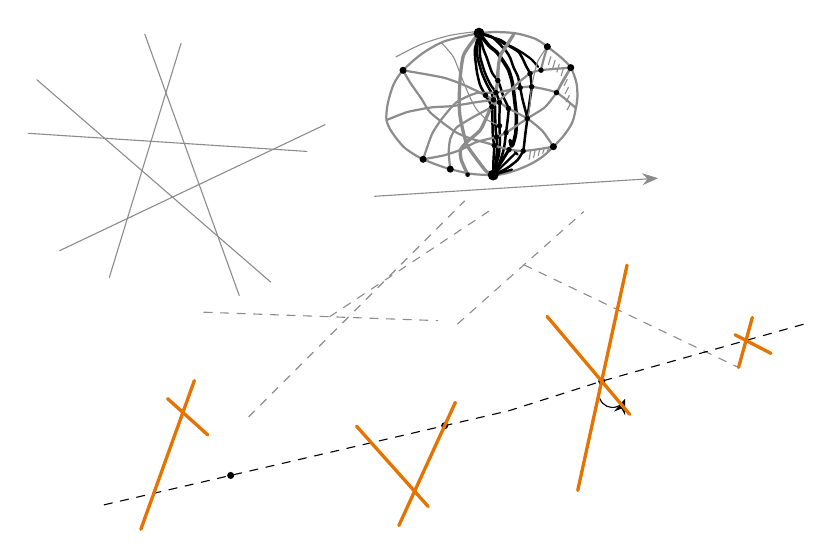
\begin{tikzpicture}[x=1mm,y=1mm,line cap=round,line join=round,font=\scriptsize]
\draw[pencil] (1.7,-6.9) -- (31.4,-32.6);
\draw[pencil] (15.4,-1.1) -- (27.4,-34.3);
\draw[pencil] (20,-2.3) -- (10.9,-32);
\draw[pencil] (4.6,-28.6) -- (38.3,-12.6);
\draw[pencil] (0.6,-13.7) -- (36,-16);
\draw[pencil,thick] plot[smooth, tension=0.5] coordinates {(57.85,-0.98) (53.5,-2) (50.6,-3.6) (48.2,-5.7) (47,-7.5) (46.25,-10) (46.1,-12) (46.75,-13.5) (48.25,-15.4) (49.8,-16.5) (50.75,-17) (52.5,-17.7) (54.2,-18.25) (56.9,-18.85) (59.65,-19) (61,-18.85) (62.8,-18.3) (64.6,-17.5) (66,-16.6) (67.3,-15.4) (68.65,-13.95) (69.7,-12.3) (70.15,-10.5) (70.35,-9) (70.2,-7.2) (69.5,-5.36) (68.3,-4.1) (66.53,-2.7) (65,-1.7) (62.5,-1) (59.9,-0.84) (57.85,-0.98)};
\draw[pencil,thin] plot[smooth, tension=0.5] coordinates {(47.3,-4) (50.5,-2.4) (54,-1.3) (57.3,-0.8)};
\draw[line width=0.9pt] plot[smooth, tension=0.4] coordinates {(57.85,-0.98) (57.33,-3) (57.35,-4) (57.6,-6) (58,-7.6) (58.68,-8.88) (59.48,-10.33) (59.55,-12.2) (59.62,-14.35) (59.79,-15.25) (59.69,-17.1) (59.65,-19)};
\draw[line width=0.9pt] plot[smooth, tension=0.4] coordinates {(57.85,-0.98) (57.6,-3) (57.65,-4) (58.2,-6) (58.85,-7.5) (59.45,-8.6) (59.69,-9.45) (59.9,-10.4) (59.9,-11.6) (59.97,-13.3) (60.07,-14.17) (60.15,-15.7) (59.95,-17.5) (59.65,-19)};
\draw[line width=0.9pt] plot[smooth, tension=0.4] coordinates {(57.85,-0.98) (57.95,-2.5) (58,-4) (58.6,-6) (59.3,-7.5) (60,-8.53) (60.45,-9.78) (60.45,-11.2) (60.45,-12.75) (60.5,-14.35) (60.38,-16.4) (59.65,-19)};
\draw[line width=0.9pt] plot[smooth, tension=0.4] coordinates {(57.85,-0.98) (58.4,-3) (58.8,-4) (59.5,-6) (60.24,-7) (60.65,-8.1) (61,-9.2) (61.59,-10.54) (61.5,-11.9) (61.28,-13.62) (61,-15.7) (60.4,-17.6) (59.65,-19)};
\draw[line width=1.3pt] plot[smooth, tension=0.4] coordinates {(57.85,-0.98) (59.13,-2.58) (60.1,-3.4) (61,-4.65) (61.62,-5.7) (62.04,-7.08) (62.25,-8.46) (62.46,-10.2) (62.6,-11.6) (62.52,-13.65) (62.18,-15.04) (61.97,-15.3) (61.8,-14.6)};
\draw[line width=0.9pt] plot[smooth, tension=0.4] coordinates {(57.85,-0.98) (59.4,-1.4) (60.4,-2.3) (61.3,-3.27) (61.8,-4.1) (62.25,-5.35) (62.75,-6.4) (63,-7.4) (63.08,-7.91) (63.4,-9.5) (63.85,-11.2) (63.98,-11.82) (63.75,-13.65) (63.55,-15.4) (63.46,-15.94) (62.73,-17.1) (61.35,-18.16) (59.65,-19)};
\draw[line width=0.9pt] plot[smooth, tension=0.4] coordinates {(57.85,-0.98) (60,-1.7) (61,-2.3) (62,-2.8) (62.9,-3.4) (63.4,-4.24) (63.85,-5.2) (64.33,-6.11) (64.53,-7.79) (64.3,-9.5) (63.98,-11.82)};
\draw[thick] plot[smooth, tension=0.4] coordinates {(57.85,-0.98) (60.6,-1.85) (61.4,-2.4) (62.4,-2.9) (63.4,-3.5) (64.5,-4.3) (65.35,-5.25)};
\draw[line width=1.1pt] (59.65,-19) -- (61.66,-15.77);
\draw[thick] (59.65,-19) -- (62.55,-16.15);
\draw[thick] (62.4,-16) -- (62.75,-16.4);
\draw[thick] (59.65,-19) -- (62.05,-18.3);
\draw[pencil,thick] plot[smooth, tension=0.4] coordinates {(48.2,-5.7) (53.33,-6.63) (56.13,-7.65) (58.68,-8.88) (59.69,-9.45) (60.45,-9.78) (61.59,-10.54) (63.98,-11.82) (65.9,-13.4) (67.3,-15.4)};
\draw[pencil,thick] plot[smooth, tension=0.4] coordinates {(48.2,-5.7) (49.1,-7.25) (50.6,-9.4) (51.7,-11.1) (54.8,-13.5) (56.9,-14.4) (59.1,-15) (59.79,-15.25) (61.66,-15.77) (63.46,-15.94) (65.5,-15.7) (67.3,-15.4)};
\draw[pencil,thick] plot[smooth, tension=0.4] coordinates {(50.75,-17) (51,-16.25) (51.9,-13.75) (53.1,-11.9) (55,-9.75) (57.5,-8.6) (60,-8.53) (63.08,-7.91) (64.53,-7.79) (67.69,-8.53) (70.15,-10.5)};
\draw[pencil,thick] plot[smooth, tension=0.4] coordinates {(50.75,-17) (53.4,-16.5) (55.5,-15.8) (57.4,-14.85) (59.1,-14.4) (60.07,-14.17) (61.28,-13.62) (63.98,-11.82) (66.2,-10.4) (67.69,-8.53) (69.5,-5.36)};
\draw[pencil,thick] plot[smooth, tension=0.4] coordinates {(54.2,-18.25) (54,-16.1) (54.2,-14.4) (54.9,-13.06) (56.06,-12.26) (57.43,-11.46) (59.48,-10.33) (61,-9) (62.7,-7.4) (64.33,-6.11) (65.72,-5.68) (69.5,-5.36)};
\draw[pencil,thick] plot[smooth, tension=0.4] coordinates {(46.15,-12) (48.75,-11) (51.9,-10.4) (54.4,-10.25) (57.5,-9.75) (59.69,-9.45)};
\draw[pencil] plot[smooth, tension=0.4] coordinates {(53.1,-2.2) (54.6,-4) (55.6,-6.5) (56.6,-8.9) (57.5,-10.6) (58.75,-11.9) (60.45,-12.75)};
\draw[pencil,line width=1.2pt] plot[smooth, tension=0.4] coordinates {(62.3,-1.05) (61.35,-2.58) (60.66,-3.6) (60.38,-4.65) (60.24,-6.04) (60.24,-7) (60.03,-8.1) (59.6,-9.9) (59.1,-11) (58,-13.3) (56.3,-14.8) (55.5,-15.8) (55.6,-17.1) (56.4,-18.9)};
\draw[pencil,line width=1.2pt] plot[smooth, tension=0.4] coordinates {(57.85,-0.98) (55.9,-3.75) (55.4,-7.5) (55.4,-11.25) (56.25,-15) (57.5,-16.9) (58.75,-18.5) (59.65,-19)};
\node[pt,pt,inner sep=0.6pt] at (56.4,-18.95) {};
\draw[pencil,thick] plot[smooth, tension=0.4] coordinates {(66.53,-2.7) (66,-4.5) (65.72,-5.68)};
\draw[pencil] plot[smooth, tension=0.4] coordinates {(66.53,-2.7) (65.3,-4.6) (64.53,-7.79) (64.3,-10.3) (63.98,-11.82)};
\draw[pencil,thick] plot[smooth, tension=0.4] coordinates {(69.5,-5.36) (68.5,-7) (67.69,-8.53)};
\draw[pencil] (64.41,-15.91) -- (64.21,-17.01);
\draw[pencil] (64.99,-15.81) -- (64.79,-16.76);
\draw[pencil] (65.57,-15.71) -- (65.37,-16.51);
\draw[pencil] (66.14,-15.6) -- (65.94,-16.25);
\draw[pencil] (66.72,-15.5) -- (66.52,-16);
\draw[pencil] (66.97,-3.97) -- (66.67,-4.96);
\draw[pencil] (67.51,-4.44) -- (67.21,-5.44);
\draw[pencil] (68.04,-4.92) -- (67.74,-5.92);
\draw[pencil] (68.58,-5.4) -- (68.28,-6.4);
\draw[pencil] (69.06,-6.85) -- (68.66,-7.65);
\draw[pencil] (69.19,-7.87) -- (68.79,-8.67);
\draw[pencil] (69.32,-8.9) -- (68.92,-9.7);
\draw[pencil] (69.45,-9.93) -- (69.05,-10.73);
\node[pt,pt,inner sep=1.4pt] at (57.85,-0.98) {};
\node[pt,pt,inner sep=1.4pt] at (59.65,-19) {};
\node[pt,pt] at (48.2,-5.7) {};
\node[pt,pt] at (50.75,-17) {};
\node[pt,pt] at (54.2,-18.25) {};
\node[pt,pt] at (66.53,-2.7) {};
\node[pt,pt] at (69.5,-5.36) {};
\node[pt,pt] at (67.3,-15.4) {};
\node[pt,pt,inner sep=0.7pt] at (58.68,-8.88) {};
\node[pt,pt,inner sep=0.7pt] at (59.69,-9.45) {};
\node[pt,pt,inner sep=0.7pt] at (59.48,-10.33) {};
\node[pt,pt,inner sep=0.7pt] at (60,-8.53) {};
\node[pt,pt,inner sep=0.7pt] at (60.24,-7) {};
\node[pt,pt,inner sep=0.7pt] at (60.45,-9.78) {};
\node[pt,pt,inner sep=0.7pt] at (61.59,-10.54) {};
\node[pt,pt,inner sep=0.7pt] at (60.45,-12.75) {};
\node[pt,pt,inner sep=0.7pt] at (61.28,-13.62) {};
\node[pt,pt,inner sep=0.7pt] at (60.07,-14.17) {};
\node[pt,pt,inner sep=0.7pt] at (59.79,-15.25) {};
\node[pt,pt,inner sep=0.7pt] at (61.66,-15.77) {};
\node[pt,pt,inner sep=0.7pt] at (63.46,-15.94) {};
\node[pt,pt,inner sep=0.7pt] at (63.98,-11.82) {};
\node[pt,pt,inner sep=0.7pt] at (63.08,-7.91) {};
\node[pt,pt,inner sep=0.7pt] at (64.53,-7.79) {};
\node[pt,pt,inner sep=0.7pt] at (64.33,-6.11) {};
\node[pt,pt,inner sep=0.7pt] at (65.72,-5.68) {};
\node[pt,pt,inner sep=0.7pt] at (67.69,-8.53) {};
\draw[pencil,-{Stealth[length=2mm]}] (44.6,-21.7) -- (80.6,-19.4);
\draw[pencil,dashed] (28.6,-49.7) -- (56,-22.3);
\draw[pencil,dashed] (38.89,-36.99) -- (59.4,-23.4);
\draw[pencil,dashed] (22.91,-36.42) -- (52.61,-37.49);
\draw[pencil,dashed] (55.11,-37.93) -- (71.13,-23.66);
\draw[pencil,dashed] (63.56,-30.41) -- (90.81,-43.44);
\draw[dashed] (10.25,-60.88) -- (61.66,-48.93) -- (73.43,-45.18) -- (99.44,-37.84);
\node[pt] at (73.43,-45.18) {};
\draw[-{Stealth[length=2mm]}] (73.2,-47.4) arc[start angle=200, end angle=340, x radius=1.7, y radius=1.7];
\node[pt] at (26.31,-57.15) {};
\node[pt] at (53.49,-50.83) {};
\draw[Or,very thick] (14.9,-64) -- (21.7,-45.1);
\draw[Or,very thick] (18.3,-47.4) -- (23.4,-52);
\draw[Or,very thick] (42.3,-50.9) -- (51.4,-61.1);
\draw[Or,very thick] (54.85,-47.86) -- (47.67,-63.51);
\draw[Or,very thick] (66.49,-36.95) -- (76.98,-49.39);
\draw[Or,very thick] (76.65,-30.44) -- (70.39,-59.05);
\draw[Or,very thick] (90.36,-39.28) -- (94.93,-41.65);
\draw[Or,very thick] (92.56,-37.09) -- (90.81,-43.44);
\end{tikzpicture}
\end{document}
